\documentclass[1p]{elsarticle_modified}
%\bibliographystyle{elsarticle-num}

%\usepackage[colorlinks]{hyperref}
%\usepackage{abbrmath_seonhwa} %\Abb, \Ascr, \Acal ,\Abf, \Afrak
\usepackage{amsfonts}
\usepackage{amssymb}
\usepackage{amsmath}
\usepackage{amsthm}
\usepackage{scalefnt}
\usepackage{amsbsy}
\usepackage{kotex}
\usepackage{caption}
\usepackage{subfig}
\usepackage{color}
\usepackage{graphicx}
\usepackage{xcolor} %% white, black, red, green, blue, cyan, magenta, yellow
\usepackage{float}
\usepackage{setspace}
\usepackage{hyperref}

\usepackage{tikz}
\usetikzlibrary{arrows}

\usepackage{multirow}
\usepackage{array} % fixed length table
\usepackage{hhline}

%%%%%%%%%%%%%%%%%%%%%
\makeatletter
\renewcommand*\env@matrix[1][\arraystretch]{%
	\edef\arraystretch{#1}%
	\hskip -\arraycolsep
	\let\@ifnextchar\new@ifnextchar
	\array{*\c@MaxMatrixCols c}}
\makeatother %https://tex.stackexchange.com/questions/14071/how-can-i-increase-the-line-spacing-in-a-matrix
%%%%%%%%%%%%%%%

\usepackage[normalem]{ulem}

\newcommand{\msout}[1]{\ifmmode\text{\sout{\ensuremath{#1}}}\else\sout{#1}\fi}
%SOURCE: \msout is \stkout macro in https://tex.stackexchange.com/questions/20609/strikeout-in-math-mode

\newcommand{\cancel}[1]{
	\ifmmode
	{\color{red}\msout{#1}}
	\else
	{\color{red}\sout{#1}}
	\fi
}

\newcommand{\add}[1]{
	{\color{blue}\uwave{#1}}
}

\newcommand{\replace}[2]{
	\ifmmode
	{\color{red}\msout{#1}}{\color{blue}\uwave{#2}}
	\else
	{\color{red}\sout{#1}}{\color{blue}\uwave{#2}}
	\fi
}

\newcommand{\Sol}{\mathcal{S}} %segment
\newcommand{\D}{D} %diagram
\newcommand{\A}{\mathcal{A}} %arc


%%%%%%%%%%%%%%%%%%%%%%%%%%%%%5 test

\def\sl{\operatorname{\textup{SL}}(2,\Cbb)}
\def\psl{\operatorname{\textup{PSL}}(2,\Cbb)}
\def\quan{\mkern 1mu \triangleright \mkern 1mu}

\theoremstyle{definition}
\newtheorem{thm}{Theorem}[section]
\newtheorem{prop}[thm]{Proposition}
\newtheorem{lem}[thm]{Lemma}
\newtheorem{ques}[thm]{Question}
\newtheorem{cor}[thm]{Corollary}
\newtheorem{defn}[thm]{Definition}
\newtheorem{exam}[thm]{Example}
\newtheorem{rmk}[thm]{Remark}
\newtheorem{alg}[thm]{Algorithm}

\newcommand{\I}{\sqrt{-1}}
\begin{document}

%\begin{frontmatter}
%
%\title{Boundary parabolic representations of knots up to 8 crossings}
%
%%% Group authors per affiliation:
%\author{Yunhi Cho} 
%\address{Department of Mathematics, University of Seoul, Seoul, Korea}
%\ead{yhcho@uos.ac.kr}
%
%
%\author{Seonhwa Kim} %\fnref{s_kim}}
%\address{Center for Geometry and Physics, Institute for Basic Science, Pohang, 37673, Korea}
%\ead{ryeona17@ibs.re.kr}
%
%\author{Hyuk Kim}
%\address{Department of Mathematical Sciences, Seoul National University, Seoul 08826, Korea}
%\ead{hyukkim@snu.ac.kr}
%
%\author{Seokbeom Yoon}
%\address{Department of Mathematical Sciences, Seoul National University, Seoul, 08826,  Korea}
%\ead{sbyoon15@snu.ac.kr}
%
%\begin{abstract}
%We find all boundary parabolic representation of knots up to 8 crossings.
%
%\end{abstract}
%\begin{keyword}
%    \MSC[2010] 57M25 
%\end{keyword}
%
%\end{frontmatter}

%\linenumbers
%\tableofcontents
%
\newcommand\colored[1]{\textcolor{white}{\rule[-0.35ex]{0.8em}{1.4ex}}\kern-0.8em\color{red} #1}%
%\newcommand\colored[1]{\textcolor{white}{ #1}\kern-2.17ex	\textcolor{white}{ #1}\kern-1.81ex	\textcolor{white}{ #1}\kern-2.15ex\color{red}#1	}

{\Large $\underline{10_{63}~(K10a_{51})}$}

\setlength{\tabcolsep}{10pt}
\renewcommand{\arraystretch}{1.6}
\vspace{1cm}\begin{tabular}{m{100pt}>{\centering\arraybackslash}m{274pt}}
\multirow{5}{120pt}{
	\centering
	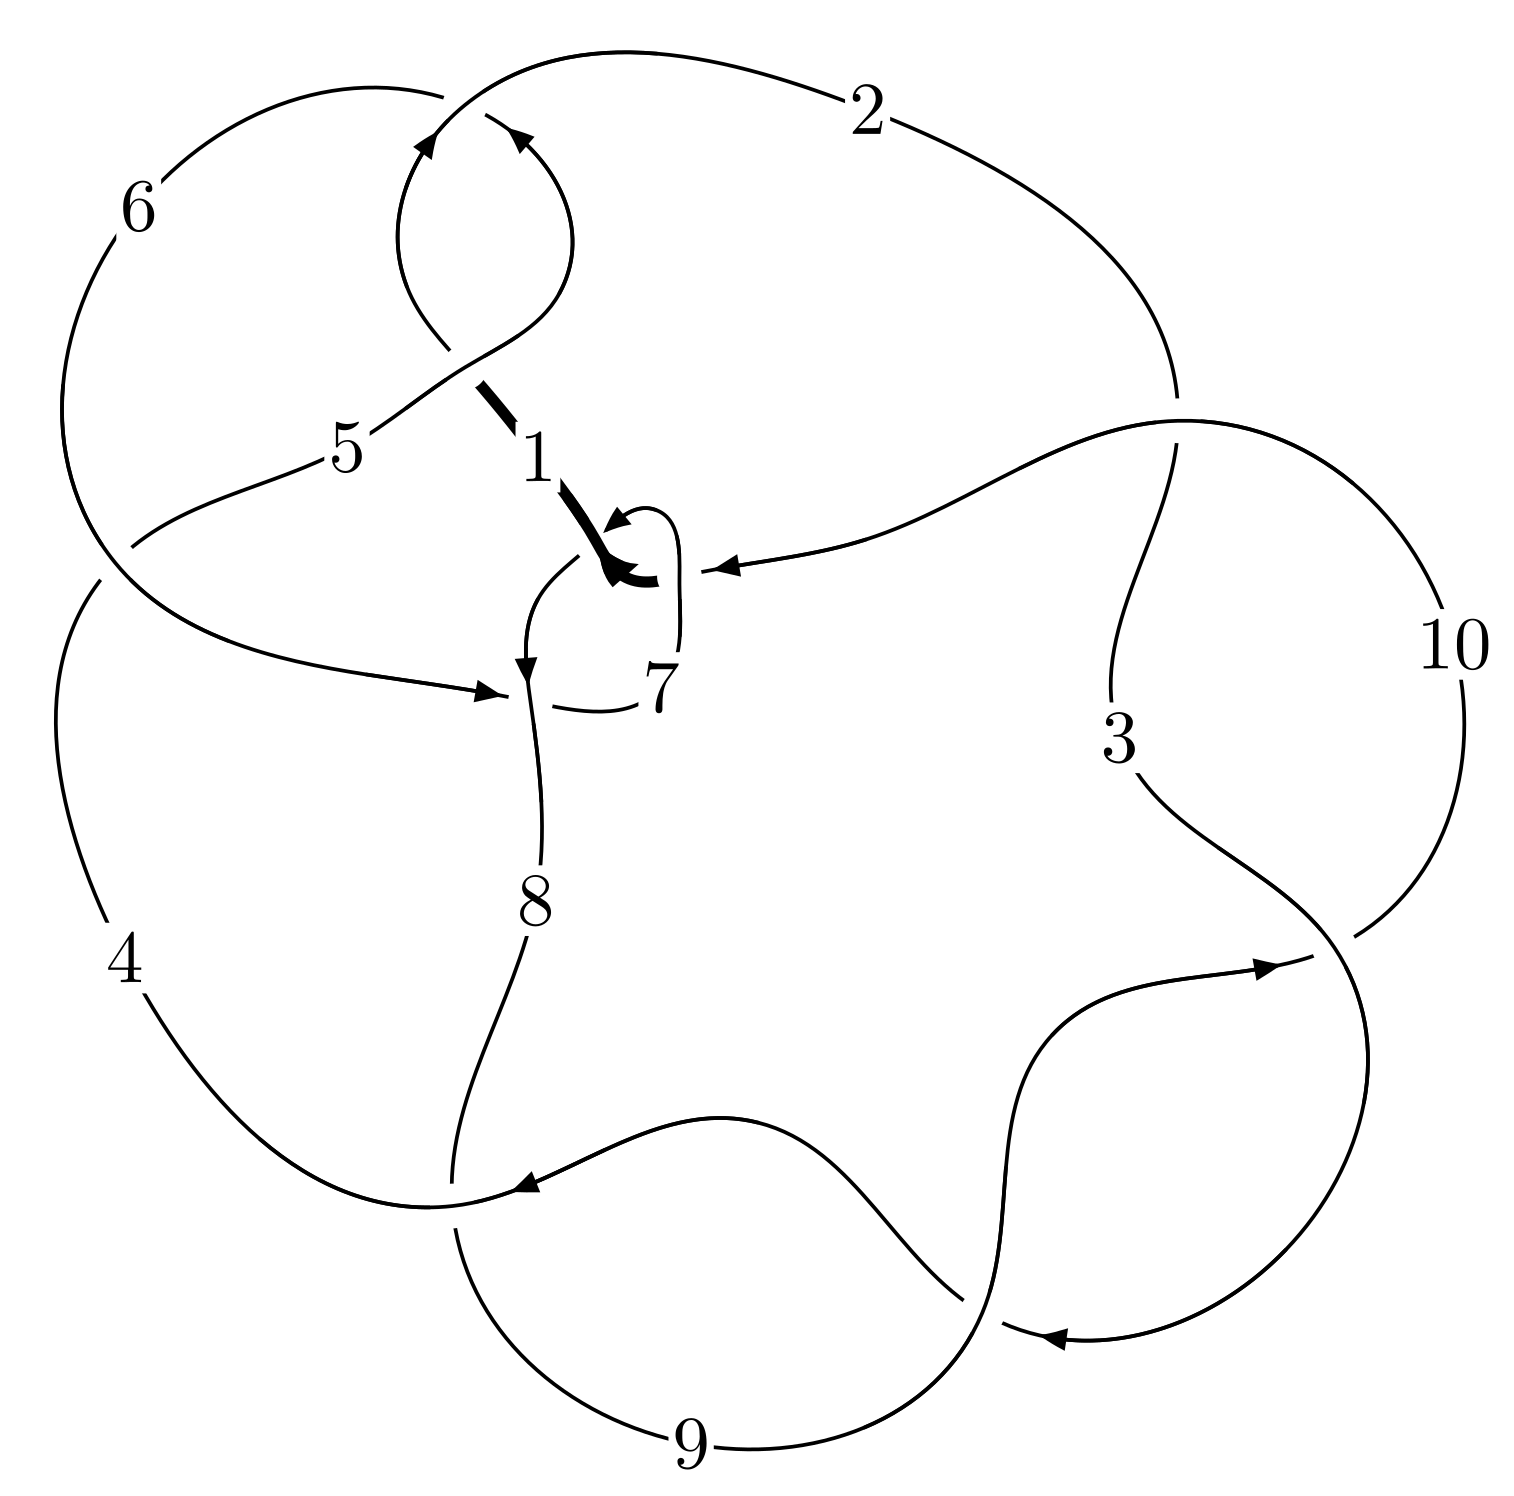
\includegraphics[width=112pt]{../../../GIT/diagram.site/Diagrams/png/147_10_63.png}\\
\ \ \ A knot diagram\footnotemark}&
\allowdisplaybreaks
\textbf{Linearized knot diagam} \\
\cline{2-2}
 &
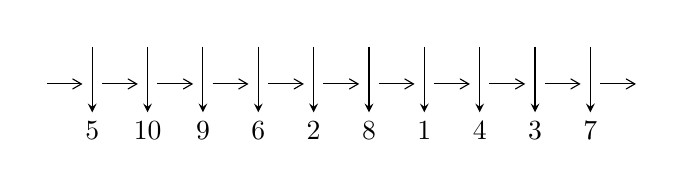
\begin{tikzpicture}[x=20pt, y=17pt]
	% nodes
	\node (C0) at (0, 0) {};
	\node (C1) at (1, 0) {};
	\node (C1U) at (1, +1) {};
	\node (C1D) at (1, -1) {5};

	\node (C2) at (2, 0) {};
	\node (C2U) at (2, +1) {};
	\node (C2D) at (2, -1) {10};

	\node (C3) at (3, 0) {};
	\node (C3U) at (3, +1) {};
	\node (C3D) at (3, -1) {9};

	\node (C4) at (4, 0) {};
	\node (C4U) at (4, +1) {};
	\node (C4D) at (4, -1) {6};

	\node (C5) at (5, 0) {};
	\node (C5U) at (5, +1) {};
	\node (C5D) at (5, -1) {2};

	\node (C6) at (6, 0) {};
	\node (C6U) at (6, +1) {};
	\node (C6D) at (6, -1) {8};

	\node (C7) at (7, 0) {};
	\node (C7U) at (7, +1) {};
	\node (C7D) at (7, -1) {1};

	\node (C8) at (8, 0) {};
	\node (C8U) at (8, +1) {};
	\node (C8D) at (8, -1) {4};

	\node (C9) at (9, 0) {};
	\node (C9U) at (9, +1) {};
	\node (C9D) at (9, -1) {3};

	\node (C10) at (10, 0) {};
	\node (C10U) at (10, +1) {};
	\node (C10D) at (10, -1) {7};
	\node (C11) at (11, 0) {};

	% arrows
	\draw[->,>={angle 60}]
	(C0) edge (C1) (C1) edge (C2) (C2) edge (C3) (C3) edge (C4) (C4) edge (C5) (C5) edge (C6) (C6) edge (C7) (C7) edge (C8) (C8) edge (C9) (C9) edge (C10) (C10) edge (C11) ;	\draw[->,>=stealth]
	(C1U) edge (C1D) (C2U) edge (C2D) (C3U) edge (C3D) (C4U) edge (C4D) (C5U) edge (C5D) (C6U) edge (C6D) (C7U) edge (C7D) (C8U) edge (C8D) (C9U) edge (C9D) (C10U) edge (C10D) ;
	\end{tikzpicture} \\
\hhline{~~} \\& 
\textbf{Solving Sequence} \\ \cline{2-2} 
 &
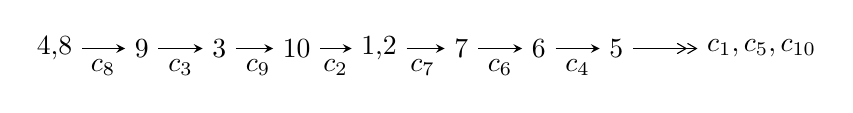
\begin{tikzpicture}[x=28pt, y=7pt]
	% node
	\node (A0) at (-1/8, 0) {4,8};
	\node (A1) at (1, 0) {9};
	\node (A2) at (2, 0) {3};
	\node (A3) at (3, 0) {10};
	\node (A4) at (65/16, 0) {1,2};
	\node (A5) at (41/8, 0) {7};
	\node (A6) at (49/8, 0) {6};
	\node (A7) at (57/8, 0) {5};
	\node (C1) at (1/2, -1) {$c_{8}$};
	\node (C2) at (3/2, -1) {$c_{3}$};
	\node (C3) at (5/2, -1) {$c_{9}$};
	\node (C4) at (7/2, -1) {$c_{2}$};
	\node (C5) at (37/8, -1) {$c_{7}$};
	\node (C6) at (45/8, -1) {$c_{6}$};
	\node (C7) at (53/8, -1) {$c_{4}$};
	\node (A8) at (9, 0) {$c_{1},c_{5},c_{10}$};

	% edge
	\draw[->,>=stealth]	
	(A0) edge (A1) (A1) edge (A2) (A2) edge (A3) (A3) edge (A4) (A4) edge (A5) (A5) edge (A6) (A6) edge (A7) ;
	\draw[->>,>={angle 60}]	
	(A7) edge (A8);
\end{tikzpicture} \\ 

\end{tabular} \\

\footnotetext{
The image of knot diagram is generated by the software ``\textbf{Draw programme}" developed by Andrew Bartholomew(\url{http://www.layer8.co.uk/maths/draw/index.htm\#Running-draw}), where we modified some parts for our purpose(\url{https://github.com/CATsTAILs/LinksPainter}).
}\phantom \\ \newline 
\centering \textbf{Ideals for irreducible components\footnotemark of $X_{\text{par}}$} 
 
\begin{align*}
I^u_{1}&=\langle 
u^{12}+2 u^{11}+9 u^{10}+14 u^9+29 u^8+34 u^7+40 u^6+32 u^5+20 u^4+7 u^3- u^2+b-2 u-1,\\
\phantom{I^u_{1}}&\phantom{= \langle  }- u^{12}-3 u^{11}-10 u^{10}-21 u^9-35 u^8-51 u^7-52 u^6-48 u^5-29 u^4-11 u^3-2 u^2+2 a+2 u,\\
\phantom{I^u_{1}}&\phantom{= \langle  }u^{13}+3 u^{12}+12 u^{11}+25 u^{10}+51 u^9+75 u^8+96 u^7+96 u^6+77 u^5+45 u^4+16 u^3-4 u-2\rangle \\
I^u_{2}&=\langle 
-2 u^8 a+2 u^8+\cdots-4 a+3,\\
\phantom{I^u_{2}}&\phantom{= \langle  }- u^7+u^5 a+u^6-2 u^4 a-5 u^5+4 u^3 a+5 u^4-6 u^2 a-8 u^3+a^2+3 a u+7 u^2-2 a-4 u+2,\\
\phantom{I^u_{2}}&\phantom{= \langle  }u^9- u^8+6 u^7-5 u^6+11 u^5-7 u^4+6 u^3-2 u^2+u-1\rangle \\
I^u_{3}&=\langle 
b+1,\;2 a- u,\;u^2+2\rangle \\
\\
I^v_{1}&=\langle 
a,\;b-1,\;v+1\rangle \\
\end{align*}
\raggedright * 4 irreducible components of $\dim_{\mathbb{C}}=0$, with total 34 representations.\\
\footnotetext{All coefficients of polynomials are rational numbers. But the coefficients are sometimes approximated in decimal forms when there is not enough margin.}
\newpage
\renewcommand{\arraystretch}{1}
\centering \section*{I. $I^u_{1}= \langle u^{12}+2 u^{11}+\cdots+b-1,\;- u^{12}-3 u^{11}+\cdots+2 a+2 u,\;u^{13}+3 u^{12}+\cdots-4 u-2 \rangle$}
\flushleft \textbf{(i) Arc colorings}\\
\begin{tabular}{m{7pt} m{180pt} m{7pt} m{180pt} }
\flushright $a_{4}=$&$\begin{pmatrix}0\\u\end{pmatrix}$ \\
\flushright $a_{8}=$&$\begin{pmatrix}1\\0\end{pmatrix}$ \\
\flushright $a_{9}=$&$\begin{pmatrix}1\\u^2\end{pmatrix}$ \\
\flushright $a_{3}=$&$\begin{pmatrix}u\\u^3+u\end{pmatrix}$ \\
\flushright $a_{10}=$&$\begin{pmatrix}u^2+1\\u^4+2 u^2\end{pmatrix}$ \\
\flushright $a_{1}=$&$\begin{pmatrix}\frac{1}{2} u^{12}+\frac{3}{2} u^{11}+\cdots+u^2- u\\- u^{12}-2 u^{11}+\cdots+2 u+1\end{pmatrix}$ \\
\flushright $a_{2}=$&$\begin{pmatrix}u^3+2 u\\u^5+3 u^3+u\end{pmatrix}$ \\
\flushright $a_{7}=$&$\begin{pmatrix}\frac{1}{2} u^{12}+\frac{3}{2} u^{11}+\cdots-2 u-1\\u^8+u^7+5 u^6+4 u^5+7 u^4+4 u^3+2 u^2-1\end{pmatrix}$ \\
\flushright $a_{6}=$&$\begin{pmatrix}\frac{1}{2} u^{12}+\frac{3}{2} u^{11}+\cdots-2 u-2\\u^8+u^7+5 u^6+4 u^5+7 u^4+4 u^3+2 u^2-1\end{pmatrix}$ \\
\flushright $a_{5}=$&$\begin{pmatrix}\frac{1}{2} u^{12}+\frac{3}{2} u^{11}+\cdots-2 u-2\\u^9+u^8+6 u^7+5 u^6+11 u^5+7 u^4+6 u^3+2 u^2+u-1\end{pmatrix}$\\&\end{tabular}
\flushleft \textbf{(ii) Obstruction class $= -1$}\\~\\
\flushleft \textbf{(iii) Cusp Shapes $= 2 u^{12}+6 u^{11}+24 u^{10}+52 u^9+100 u^8+154 u^7+174 u^6+174 u^5+108 u^4+46 u^3-4 u^2-14 u-16$}\\~\\
\newpage\renewcommand{\arraystretch}{1}
\flushleft \textbf{(iv) u-Polynomials at the component}\newline \\
\begin{tabular}{m{50pt}|m{274pt}}
Crossings & \hspace{64pt}u-Polynomials at each crossing \\
\hline $$\begin{aligned}c_{1},c_{5},c_{7}\\c_{10}\end{aligned}$$&$\begin{aligned}
&u^{13}+u^{12}+\cdots+u+1
\end{aligned}$\\
\hline $$\begin{aligned}c_{2},c_{3},c_{8}\\c_{9}\end{aligned}$$&$\begin{aligned}
&u^{13}-3 u^{12}+\cdots-4 u+2
\end{aligned}$\\
\hline $$\begin{aligned}c_{4},c_{6}\end{aligned}$$&$\begin{aligned}
&u^{13}+5 u^{12}+\cdots+9 u+1
\end{aligned}$\\
\hline
\end{tabular}\\~\\
\newpage\renewcommand{\arraystretch}{1}
\flushleft \textbf{(v) Riley Polynomials at the component}\newline \\
\begin{tabular}{m{50pt}|m{274pt}}
Crossings & \hspace{64pt}Riley Polynomials at each crossing \\
\hline $$\begin{aligned}c_{1},c_{5},c_{7}\\c_{10}\end{aligned}$$&$\begin{aligned}
&y^{13}-5 y^{12}+\cdots+9 y-1
\end{aligned}$\\
\hline $$\begin{aligned}c_{2},c_{3},c_{8}\\c_{9}\end{aligned}$$&$\begin{aligned}
&y^{13}+15 y^{12}+\cdots+16 y-4
\end{aligned}$\\
\hline $$\begin{aligned}c_{4},c_{6}\end{aligned}$$&$\begin{aligned}
&y^{13}+11 y^{12}+\cdots+25 y-1
\end{aligned}$\\
\hline
\end{tabular}\\~\\
\newpage\flushleft \textbf{(vi) Complex Volumes and Cusp Shapes}
$$\begin{array}{c|c|c}  
\text{Solutions to }I^u_{1}& \I (\text{vol} + \sqrt{-1}CS) & \text{Cusp shape}\\
 \hline 
\begin{aligned}
u &= -0.138146 + 0.948701 I \\
a &= \phantom{-}0.317222 + 0.611463 I \\
b &= -0.644264 - 0.592137 I\end{aligned}
 & \phantom{-}2.65637 - 1.35876 I & -4.47319 + 3.17078 I \\ \hline\begin{aligned}
u &= -0.138146 - 0.948701 I \\
a &= \phantom{-}0.317222 - 0.611463 I \\
b &= -0.644264 + 0.592137 I\end{aligned}
 & \phantom{-}2.65637 + 1.35876 I & -4.47319 - 3.17078 I \\ \hline\begin{aligned}
u &= -0.578420 + 0.729059 I \\
a &= -0.85431 - 1.51986 I \\
b &= -1.089570 + 0.623417 I\end{aligned}
 & -0.00714 + 8.67404 I & -9.53036 - 8.43648 I \\ \hline\begin{aligned}
u &= -0.578420 - 0.729059 I \\
a &= -0.85431 + 1.51986 I \\
b &= -1.089570 - 0.623417 I\end{aligned}
 & -0.00714 - 8.67404 I & -9.53036 + 8.43648 I \\ \hline\begin{aligned}
u &= -0.694065 + 0.222366 I \\
a &= \phantom{-}0.835992 + 0.144863 I \\
b &= \phantom{-}0.982157 + 0.559210 I\end{aligned}
 & -1.52198 - 4.38846 I & -11.77625 + 4.32757 I \\ \hline\begin{aligned}
u &= -0.694065 - 0.222366 I \\
a &= \phantom{-}0.835992 - 0.144863 I \\
b &= \phantom{-}0.982157 - 0.559210 I\end{aligned}
 & -1.52198 + 4.38846 I & -11.77625 - 4.32757 I \\ \hline\begin{aligned}
u &= -0.063059 + 1.278080 I \\
a &= -0.069487 + 0.291937 I \\
b &= -0.750183 - 0.366139 I\end{aligned}
 & \phantom{-}2.83101 - 1.40076 I & -6.04773 + 4.90140 I \\ \hline\begin{aligned}
u &= -0.063059 - 1.278080 I \\
a &= -0.069487 - 0.291937 I \\
b &= -0.750183 + 0.366139 I\end{aligned}
 & \phantom{-}2.83101 + 1.40076 I & -6.04773 - 4.90140 I \\ \hline\begin{aligned}
u &= \phantom{-}0.400549\phantom{ +0.000000I} \\
a &= \phantom{-}0.898581\phantom{ +0.000000I} \\
b &= \phantom{-}0.421510\phantom{ +0.000000I}\end{aligned}
 & -0.714503\phantom{ +0.000000I} & -13.6630\phantom{ +0.000000I} \\ \hline\begin{aligned}
u &= -0.17430 + 1.61896 I \\
a &= -0.03628 + 1.72509 I \\
b &= \phantom{-}1.168160 - 0.683587 I\end{aligned}
 & \phantom{-}7.93590 + 11.51170 I & -7.17210 - 6.84034 I\\
 \hline 
 \end{array}$$\newpage$$\begin{array}{c|c|c}  
\text{Solutions to }I^u_{1}& \I (\text{vol} + \sqrt{-1}CS) & \text{Cusp shape}\\
 \hline 
\begin{aligned}
u &= -0.17430 - 1.61896 I \\
a &= -0.03628 - 1.72509 I \\
b &= \phantom{-}1.168160 + 0.683587 I\end{aligned}
 & \phantom{-}7.93590 - 11.51170 I & -7.17210 + 6.84034 I \\ \hline\begin{aligned}
u &= -0.05229 + 1.64838 I \\
a &= -0.642426 - 1.259340 I \\
b &= \phantom{-}0.622947 + 0.904317 I\end{aligned}
 & \phantom{-}11.49220 - 0.51506 I & -3.16885 + 2.03529 I \\ \hline\begin{aligned}
u &= -0.05229 - 1.64838 I \\
a &= -0.642426 + 1.259340 I \\
b &= \phantom{-}0.622947 - 0.904317 I\end{aligned}
 & \phantom{-}11.49220 + 0.51506 I & -3.16885 - 2.03529 I\\
 \hline 
 \end{array}$$\newpage\newpage\renewcommand{\arraystretch}{1}
\centering \section*{II. $I^u_{2}= \langle -2 u^8 a+2 u^8+\cdots-4 a+3,\;- u^7+u^6+\cdots-2 a+2,\;u^9- u^8+\cdots+u-1 \rangle$}
\flushleft \textbf{(i) Arc colorings}\\
\begin{tabular}{m{7pt} m{180pt} m{7pt} m{180pt} }
\flushright $a_{4}=$&$\begin{pmatrix}0\\u\end{pmatrix}$ \\
\flushright $a_{8}=$&$\begin{pmatrix}1\\0\end{pmatrix}$ \\
\flushright $a_{9}=$&$\begin{pmatrix}1\\u^2\end{pmatrix}$ \\
\flushright $a_{3}=$&$\begin{pmatrix}u\\u^3+u\end{pmatrix}$ \\
\flushright $a_{10}=$&$\begin{pmatrix}u^2+1\\u^4+2 u^2\end{pmatrix}$ \\
\flushright $a_{1}=$&$\begin{pmatrix}a\\2 u^8 a-2 u^8+\cdots+4 a-3\end{pmatrix}$ \\
\flushright $a_{2}=$&$\begin{pmatrix}u^3+2 u\\u^5+3 u^3+u\end{pmatrix}$ \\
\flushright $a_{7}=$&$\begin{pmatrix}-2 u^8 a+2 u^8+\cdots-3 a+3\\-3 u^8 a+3 u^8+\cdots-5 a+4\end{pmatrix}$ \\
\flushright $a_{6}=$&$\begin{pmatrix}-5 u^8 a+5 u^8+\cdots-8 a+7\\-3 u^8 a+3 u^8+\cdots-5 a+4\end{pmatrix}$ \\
\flushright $a_{5}=$&$\begin{pmatrix}2 u^8 a-2 u^8+\cdots+3 a-2\\1\end{pmatrix}$\\&\end{tabular}
\flushleft \textbf{(ii) Obstruction class $= -1$}\\~\\
\flushleft \textbf{(iii) Cusp Shapes $= -4 u^7+4 u^6-20 u^5+16 u^4-28 u^3+16 u^2-8 u-6$}\\~\\
\newpage\renewcommand{\arraystretch}{1}
\flushleft \textbf{(iv) u-Polynomials at the component}\newline \\
\begin{tabular}{m{50pt}|m{274pt}}
Crossings & \hspace{64pt}u-Polynomials at each crossing \\
\hline $$\begin{aligned}c_{1},c_{5},c_{7}\\c_{10}\end{aligned}$$&$\begin{aligned}
&u^{18}+u^{17}+\cdots+4 u+3
\end{aligned}$\\
\hline $$\begin{aligned}c_{2},c_{3},c_{8}\\c_{9}\end{aligned}$$&$\begin{aligned}
&(u^9+u^8+6 u^7+5 u^6+11 u^5+7 u^4+6 u^3+2 u^2+u+1)^2
\end{aligned}$\\
\hline $$\begin{aligned}c_{4},c_{6}\end{aligned}$$&$\begin{aligned}
&u^{18}+9 u^{17}+\cdots+40 u+9
\end{aligned}$\\
\hline
\end{tabular}\\~\\
\newpage\renewcommand{\arraystretch}{1}
\flushleft \textbf{(v) Riley Polynomials at the component}\newline \\
\begin{tabular}{m{50pt}|m{274pt}}
Crossings & \hspace{64pt}Riley Polynomials at each crossing \\
\hline $$\begin{aligned}c_{1},c_{5},c_{7}\\c_{10}\end{aligned}$$&$\begin{aligned}
&y^{18}-9 y^{17}+\cdots-40 y+9
\end{aligned}$\\
\hline $$\begin{aligned}c_{2},c_{3},c_{8}\\c_{9}\end{aligned}$$&$\begin{aligned}
&(y^9+11 y^8+48 y^7+105 y^6+121 y^5+73 y^4+20 y^3-6 y^2-3 y-1)^2
\end{aligned}$\\
\hline $$\begin{aligned}c_{4},c_{6}\end{aligned}$$&$\begin{aligned}
&y^{18}- y^{17}+\cdots+524 y+81
\end{aligned}$\\
\hline
\end{tabular}\\~\\
\newpage\flushleft \textbf{(vi) Complex Volumes and Cusp Shapes}
$$\begin{array}{c|c|c}  
\text{Solutions to }I^u_{2}& \I (\text{vol} + \sqrt{-1}CS) & \text{Cusp shape}\\
 \hline 
\begin{aligned}
u &= \phantom{-}0.429032 + 0.787939 I \\
a &= \phantom{-}0.559116 - 0.339074 I \\
b &= -0.444651 + 0.766223 I\end{aligned}
 & \phantom{-}1.87293 - 3.41073 I & -6.11762 + 4.39642 I \\ \hline\begin{aligned}
u &= \phantom{-}0.429032 + 0.787939 I \\
a &= -0.47019 + 1.53024 I \\
b &= -0.935577 - 0.603792 I\end{aligned}
 & \phantom{-}1.87293 - 3.41073 I & -6.11762 + 4.39642 I \\ \hline\begin{aligned}
u &= \phantom{-}0.429032 - 0.787939 I \\
a &= \phantom{-}0.559116 + 0.339074 I \\
b &= -0.444651 - 0.766223 I\end{aligned}
 & \phantom{-}1.87293 + 3.41073 I & -6.11762 - 4.39642 I \\ \hline\begin{aligned}
u &= \phantom{-}0.429032 - 0.787939 I \\
a &= -0.47019 - 1.53024 I \\
b &= -0.935577 + 0.603792 I\end{aligned}
 & \phantom{-}1.87293 + 3.41073 I & -6.11762 - 4.39642 I \\ \hline\begin{aligned}
u &= \phantom{-}0.590618\phantom{ +0.000000I} \\
a &= \phantom{-}0.834260 + 0.039950 I \\
b &= \phantom{-}0.640279 + 0.479450 I\end{aligned}
 & -0.453072\phantom{ +0.000000I} & -10.3330\phantom{ +0.000000I} \\ \hline\begin{aligned}
u &= \phantom{-}0.590618\phantom{ +0.000000I} \\
a &= \phantom{-}0.834260 - 0.039950 I \\
b &= \phantom{-}0.640279 - 0.479450 I\end{aligned}
 & -0.453072\phantom{ +0.000000I} & -10.3330\phantom{ +0.000000I} \\ \hline\begin{aligned}
u &= -0.290170 + 0.487341 I \\
a &= \phantom{-}1.066630 + 0.144171 I \\
b &= \phantom{-}1.174710 + 0.153689 I\end{aligned}
 & -3.25448 + 1.10969 I & -11.44626 - 6.23947 I \\ \hline\begin{aligned}
u &= -0.290170 + 0.487341 I \\
a &= \phantom{-}0.06769 - 3.10644 I \\
b &= -0.943806 + 0.303030 I\end{aligned}
 & -3.25448 + 1.10969 I & -11.44626 - 6.23947 I \\ \hline\begin{aligned}
u &= -0.290170 - 0.487341 I \\
a &= \phantom{-}1.066630 - 0.144171 I \\
b &= \phantom{-}1.174710 - 0.153689 I\end{aligned}
 & -3.25448 - 1.10969 I & -11.44626 + 6.23947 I \\ \hline\begin{aligned}
u &= -0.290170 - 0.487341 I \\
a &= \phantom{-}0.06769 + 3.10644 I \\
b &= -0.943806 - 0.303030 I\end{aligned}
 & -3.25448 - 1.10969 I & -11.44626 + 6.23947 I\\
 \hline 
 \end{array}$$\newpage$$\begin{array}{c|c|c}  
\text{Solutions to }I^u_{2}& \I (\text{vol} + \sqrt{-1}CS) & \text{Cusp shape}\\
 \hline 
\begin{aligned}
u &= -0.05587 + 1.55975 I \\
a &= \phantom{-}0.1256620 + 0.0280657 I \\
b &= -1.339950 - 0.113954 I\end{aligned}
 & \phantom{-}3.77376 + 2.21388 I & -7.75885 - 3.04598 I \\ \hline\begin{aligned}
u &= -0.05587 + 1.55975 I \\
a &= -0.77131 + 1.94759 I \\
b &= \phantom{-}0.857711 - 0.553032 I\end{aligned}
 & \phantom{-}3.77376 + 2.21388 I & -7.75885 - 3.04598 I \\ \hline\begin{aligned}
u &= -0.05587 - 1.55975 I \\
a &= \phantom{-}0.1256620 - 0.0280657 I \\
b &= -1.339950 + 0.113954 I\end{aligned}
 & \phantom{-}3.77376 - 2.21388 I & -7.75885 + 3.04598 I \\ \hline\begin{aligned}
u &= -0.05587 - 1.55975 I \\
a &= -0.77131 - 1.94759 I \\
b &= \phantom{-}0.857711 + 0.553032 I\end{aligned}
 & \phantom{-}3.77376 - 2.21388 I & -7.75885 + 3.04598 I \\ \hline\begin{aligned}
u &= \phantom{-}0.12170 + 1.63384 I \\
a &= -0.664164 + 1.104630 I \\
b &= \phantom{-}0.437217 - 0.966793 I\end{aligned}
 & \phantom{-}10.17130 - 5.50049 I & -4.51063 + 2.97298 I \\ \hline\begin{aligned}
u &= \phantom{-}0.12170 + 1.63384 I \\
a &= -0.24771 - 1.68585 I \\
b &= \phantom{-}1.054070 + 0.732497 I\end{aligned}
 & \phantom{-}10.17130 - 5.50049 I & -4.51063 + 2.97298 I \\ \hline\begin{aligned}
u &= \phantom{-}0.12170 - 1.63384 I \\
a &= -0.664164 - 1.104630 I \\
b &= \phantom{-}0.437217 + 0.966793 I\end{aligned}
 & \phantom{-}10.17130 + 5.50049 I & -4.51063 - 2.97298 I \\ \hline\begin{aligned}
u &= \phantom{-}0.12170 - 1.63384 I \\
a &= -0.24771 + 1.68585 I \\
b &= \phantom{-}1.054070 - 0.732497 I\end{aligned}
 & \phantom{-}10.17130 + 5.50049 I & -4.51063 - 2.97298 I\\
 \hline 
 \end{array}$$\newpage\newpage\renewcommand{\arraystretch}{1}
\centering \section*{III. $I^u_{3}= \langle b+1,\;2 a- u,\;u^2+2 \rangle$}
\flushleft \textbf{(i) Arc colorings}\\
\begin{tabular}{m{7pt} m{180pt} m{7pt} m{180pt} }
\flushright $a_{4}=$&$\begin{pmatrix}0\\u\end{pmatrix}$ \\
\flushright $a_{8}=$&$\begin{pmatrix}1\\0\end{pmatrix}$ \\
\flushright $a_{9}=$&$\begin{pmatrix}1\\-2\end{pmatrix}$ \\
\flushright $a_{3}=$&$\begin{pmatrix}u\\- u\end{pmatrix}$ \\
\flushright $a_{10}=$&$\begin{pmatrix}-1\\0\end{pmatrix}$ \\
\flushright $a_{1}=$&$\begin{pmatrix}\frac{1}{2} u\\-1\end{pmatrix}$ \\
\flushright $a_{2}=$&$\begin{pmatrix}0\\- u\end{pmatrix}$ \\
\flushright $a_{7}=$&$\begin{pmatrix}\frac{1}{2} u+1\\-1\end{pmatrix}$ \\
\flushright $a_{6}=$&$\begin{pmatrix}\frac{1}{2} u\\-1\end{pmatrix}$ \\
\flushright $a_{5}=$&$\begin{pmatrix}\frac{1}{2} u\\u-1\end{pmatrix}$\\&\end{tabular}
\flushleft \textbf{(ii) Obstruction class $= 1$}\\~\\
\flushleft \textbf{(iii) Cusp Shapes $= -12$}\\~\\
\newpage\renewcommand{\arraystretch}{1}
\flushleft \textbf{(iv) u-Polynomials at the component}\newline \\
\begin{tabular}{m{50pt}|m{274pt}}
Crossings & \hspace{64pt}u-Polynomials at each crossing \\
\hline $$\begin{aligned}c_{1},c_{7}\end{aligned}$$&$\begin{aligned}
&(u+1)^2
\end{aligned}$\\
\hline $$\begin{aligned}c_{2},c_{3},c_{8}\\c_{9}\end{aligned}$$&$\begin{aligned}
&u^2+2
\end{aligned}$\\
\hline $$\begin{aligned}c_{4},c_{5},c_{6}\\c_{10}\end{aligned}$$&$\begin{aligned}
&(u-1)^2
\end{aligned}$\\
\hline
\end{tabular}\\~\\
\newpage\renewcommand{\arraystretch}{1}
\flushleft \textbf{(v) Riley Polynomials at the component}\newline \\
\begin{tabular}{m{50pt}|m{274pt}}
Crossings & \hspace{64pt}Riley Polynomials at each crossing \\
\hline $$\begin{aligned}c_{1},c_{4},c_{5}\\c_{6},c_{7},c_{10}\end{aligned}$$&$\begin{aligned}
&(y-1)^2
\end{aligned}$\\
\hline $$\begin{aligned}c_{2},c_{3},c_{8}\\c_{9}\end{aligned}$$&$\begin{aligned}
&(y+2)^2
\end{aligned}$\\
\hline
\end{tabular}\\~\\
\newpage\flushleft \textbf{(vi) Complex Volumes and Cusp Shapes}
$$\begin{array}{c|c|c}  
\text{Solutions to }I^u_{3}& \I (\text{vol} + \sqrt{-1}CS) & \text{Cusp shape}\\
 \hline 
\begin{aligned}
u &= \phantom{-0.000000 -}1.414210 I \\
a &= \phantom{-0.000000 -}0.707107 I \\
b &= -1.00000\phantom{ +0.000000I}\end{aligned}
 & \phantom{-}1.64493\phantom{ +0.000000I} & -12.0000\phantom{ +0.000000I} \\ \hline\begin{aligned}
u &= \phantom{-0.000000 } -1.414210 I \\
a &= \phantom{-0.000000 } -0.707107 I \\
b &= -1.00000\phantom{ +0.000000I}\end{aligned}
 & \phantom{-}1.64493\phantom{ +0.000000I} & -12.0000\phantom{ +0.000000I}\\
 \hline 
 \end{array}$$\newpage\newpage\renewcommand{\arraystretch}{1}
\centering \section*{IV. $I^v_{1}= \langle a,\;b-1,\;v+1 \rangle$}
\flushleft \textbf{(i) Arc colorings}\\
\begin{tabular}{m{7pt} m{180pt} m{7pt} m{180pt} }
\flushright $a_{4}=$&$\begin{pmatrix}-1\\0\end{pmatrix}$ \\
\flushright $a_{8}=$&$\begin{pmatrix}1\\0\end{pmatrix}$ \\
\flushright $a_{9}=$&$\begin{pmatrix}1\\0\end{pmatrix}$ \\
\flushright $a_{3}=$&$\begin{pmatrix}-1\\0\end{pmatrix}$ \\
\flushright $a_{10}=$&$\begin{pmatrix}1\\0\end{pmatrix}$ \\
\flushright $a_{1}=$&$\begin{pmatrix}0\\1\end{pmatrix}$ \\
\flushright $a_{2}=$&$\begin{pmatrix}-1\\0\end{pmatrix}$ \\
\flushright $a_{7}=$&$\begin{pmatrix}1\\-1\end{pmatrix}$ \\
\flushright $a_{6}=$&$\begin{pmatrix}0\\-1\end{pmatrix}$ \\
\flushright $a_{5}=$&$\begin{pmatrix}-1\\-1\end{pmatrix}$\\&\end{tabular}
\flushleft \textbf{(ii) Obstruction class $= 1$}\\~\\
\flushleft \textbf{(iii) Cusp Shapes $= -12$}\\~\\
\newpage\renewcommand{\arraystretch}{1}
\flushleft \textbf{(iv) u-Polynomials at the component}\newline \\
\begin{tabular}{m{50pt}|m{274pt}}
Crossings & \hspace{64pt}u-Polynomials at each crossing \\
\hline $$\begin{aligned}c_{1},c_{4},c_{6}\\c_{7}\end{aligned}$$&$\begin{aligned}
&u-1
\end{aligned}$\\
\hline $$\begin{aligned}c_{2},c_{3},c_{8}\\c_{9}\end{aligned}$$&$\begin{aligned}
&u
\end{aligned}$\\
\hline $$\begin{aligned}c_{5},c_{10}\end{aligned}$$&$\begin{aligned}
&u+1
\end{aligned}$\\
\hline
\end{tabular}\\~\\
\newpage\renewcommand{\arraystretch}{1}
\flushleft \textbf{(v) Riley Polynomials at the component}\newline \\
\begin{tabular}{m{50pt}|m{274pt}}
Crossings & \hspace{64pt}Riley Polynomials at each crossing \\
\hline $$\begin{aligned}c_{1},c_{4},c_{5}\\c_{6},c_{7},c_{10}\end{aligned}$$&$\begin{aligned}
&y-1
\end{aligned}$\\
\hline $$\begin{aligned}c_{2},c_{3},c_{8}\\c_{9}\end{aligned}$$&$\begin{aligned}
&y
\end{aligned}$\\
\hline
\end{tabular}\\~\\
\newpage\flushleft \textbf{(vi) Complex Volumes and Cusp Shapes}
$$\begin{array}{c|c|c}  
\text{Solutions to }I^v_{1}& \I (\text{vol} + \sqrt{-1}CS) & \text{Cusp shape}\\
 \hline 
\begin{aligned}
v &= -1.00000\phantom{ +0.000000I} \\
a &= \phantom{-0.000000 } 0 \\
b &= \phantom{-}1.00000\phantom{ +0.000000I}\end{aligned}
 & -3.28987\phantom{ +0.000000I} & -12.0000\phantom{ +0.000000I}\\
 \hline 
 \end{array}$$\newpage
\newpage\renewcommand{\arraystretch}{1}
\centering \section*{ V. u-Polynomials}
\begin{tabular}{m{50pt}|m{274pt}}
Crossings & \hspace{64pt}u-Polynomials at each crossing \\
\hline $$\begin{aligned}c_{1},c_{7}\end{aligned}$$&$\begin{aligned}
&(u-1)(u+1)^2(u^{13}+u^{12}+\cdots+u+1)(u^{18}+u^{17}+\cdots+4 u+3)
\end{aligned}$\\
\hline $$\begin{aligned}c_{2},c_{3},c_{8}\\c_{9}\end{aligned}$$&$\begin{aligned}
&u(u^2+2)(u^9+u^8+6 u^7+5 u^6+11 u^5+7 u^4+6 u^3+2 u^2+u+1)^2\\
&\cdot(u^{13}-3 u^{12}+\cdots-4 u+2)
\end{aligned}$\\
\hline $$\begin{aligned}c_{4},c_{6}\end{aligned}$$&$\begin{aligned}
&((u-1)^3)(u^{13}+5 u^{12}+\cdots+9 u+1)(u^{18}+9 u^{17}+\cdots+40 u+9)
\end{aligned}$\\
\hline $$\begin{aligned}c_{5},c_{10}\end{aligned}$$&$\begin{aligned}
&((u-1)^2)(u+1)(u^{13}+u^{12}+\cdots+u+1)(u^{18}+u^{17}+\cdots+4 u+3)
\end{aligned}$\\
\hline
\end{tabular}\newpage\renewcommand{\arraystretch}{1}
\centering \section*{ VI. Riley Polynomials}
\begin{tabular}{m{50pt}|m{274pt}}
Crossings & \hspace{64pt}Riley Polynomials at each crossing \\
\hline $$\begin{aligned}c_{1},c_{5},c_{7}\\c_{10}\end{aligned}$$&$\begin{aligned}
&((y-1)^3)(y^{13}-5 y^{12}+\cdots+9 y-1)(y^{18}-9 y^{17}+\cdots-40 y+9)
\end{aligned}$\\
\hline $$\begin{aligned}c_{2},c_{3},c_{8}\\c_{9}\end{aligned}$$&$\begin{aligned}
&y(y+2)^2\\
&\cdot(y^9+11 y^8+48 y^7+105 y^6+121 y^5+73 y^4+20 y^3-6 y^2-3 y-1)^2\\
&\cdot(y^{13}+15 y^{12}+\cdots+16 y-4)
\end{aligned}$\\
\hline $$\begin{aligned}c_{4},c_{6}\end{aligned}$$&$\begin{aligned}
&((y-1)^3)(y^{13}+11 y^{12}+\cdots+25 y-1)(y^{18}- y^{17}+\cdots+524 y+81)
\end{aligned}$\\
\hline
\end{tabular}
\vskip 2pc
\end{document}